% Nikolai Nielsens "Fysiske Fag" preamble
\documentclass[a4paper,10pt]{article} 	% A4 papir, 10pt størrelse
\usepackage[english]{babel}
\usepackage{Nikolai} 					% Min hjemmelavede pakke
\usepackage[dvipsnames]{xcolor}
\usepackage{gensymb}

% Margen
\usepackage[margin=1in]{geometry}

% Max antal kolonner i en matrix. Default er 10
%\setcounter{MaxMatrixCols}{20}

% Hvor dybt skal kapitler labeles?
%\setcounter{secnumdepth}{4}	
%\setcounter{tocdepth}{4}


% Hvilket nummer skal der startes med i sections? (n-1)
%\setcounter{section}{0}	

% Til nummerering af ligninger. Så der står (afsnit.ligning) og ikke bare (ligning)
\numberwithin{equation}{section}


% Header
%\usepackage{fancyhdr}
%\head{}
%\pagestyle{fancy}

%Titel
\title{Numerical Methods in Physics Week 1}
\author{Nikolai Plambech Nielsen, LPK331. Version 1.0}
\date{\today}

\begin{document}
	\maketitle
	\section{Nuclear Decay}
	We have two radioactive isotopes, A and B, with populations $ N_A(t) $ and $ N_B(t) $, and decay times $ \tau_A $  and $ \tau_B $. Type A decays into type B, while B decays into something else we don't track. The relevant differential equations are
	\begin{equation}\label{key}
		\diff[\ud]{N_A}{t} = - \frac{N_A}{\tau_A}, \quad \diff[\ud]{N_B}{t} = \frac{N_A}{\tau_A} - \frac{N_B}{\tau_B}.
	\end{equation}
	The purpose of this assignment is to solve this problem numerically for a number of different conditions, using Euler integration. This method is used for its simplicity and ease of implementation. For all of the following simulations and plots, the values $ \Delta t = 0.1 $ is used.
	
	\subsection{Compare the numerical and analytical solutions}
	The analytical solutions are given in the assignment, and are as follows:
	\begin{align}
		N_A(t) &= N_A(0) \exp\pp{-\frac{t}{\tau_A}}, \\
		N_B(t) &= \begin{cases}
		N_B(0) \exp\pp{-\frac{t}{\tau_A}} + t \frac{N_A(0)}{\tau_A} \exp\pp{-\frac{t}{\tau_A}}, & \tau_A= \tau_B, \\
		N_B(0) \exp\pp{-\frac{t}{\tau_B}} + \frac{N_A(0)}{\frac{\tau_A}{\tau_B} - 1} \bb{\exp\pp{-\frac{t}{\tau_A}} - \exp\pp{-\frac{t}{\tau_B}}}, & \tau_A \neq \tau_B.
		\end{cases}
	\end{align}	
	The results, along with residual plots, for $ N_A(0) = N_B(0) = 1000 $ and $ \tau_A = 5, \tau_B = 10 $ are shown below, with the analytical solution for $ \tau_A \neq \tau_B $:
	\begin{figure}[H]
		\centering
		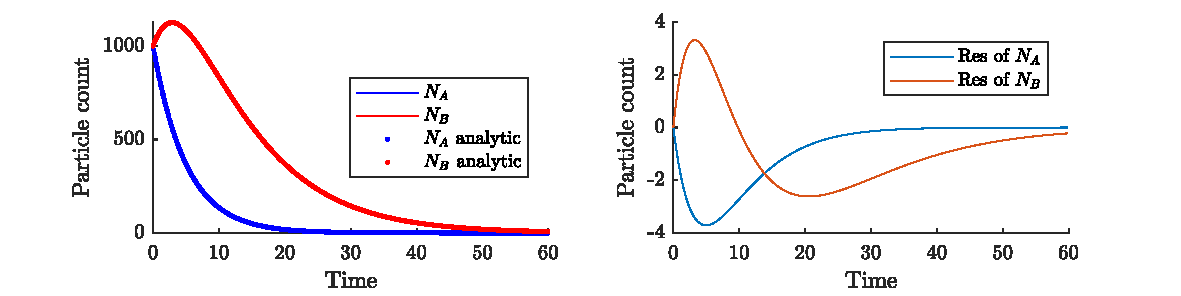
\includegraphics[width=0.7\linewidth]{unequaltau.pdf}
		\caption{\textbf{INSERT PURDY CAPTION PL0X}}
		\label{fig:unequalTau}
	\end{figure}
\textbf{COMMENT ON RESULT, YAS, V V V GUT}
	To demonstrate the solution for $ \tau_A = \tau_B $, the initial conditions of $ N_A=N_B = 1000 $ and $ \tau_A=\tau_B = 10 $ are shown below. Again with accompanying residual plots:
	\begin{figure}[H]
		\centering
		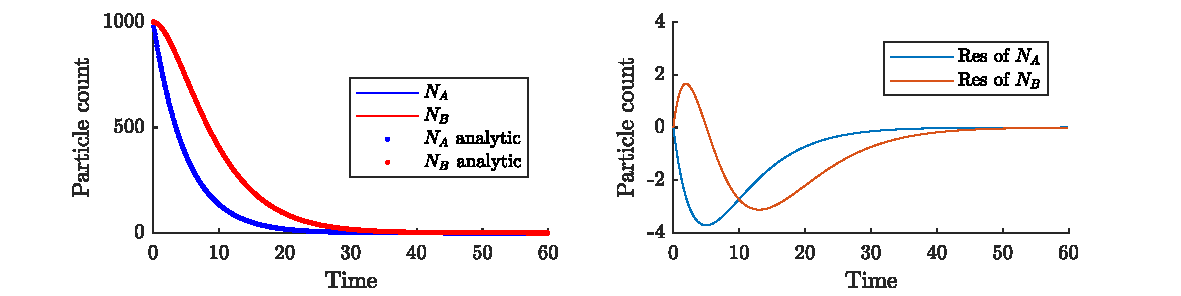
\includegraphics[width=0.7\linewidth]{equaltau.pdf}
		\caption{\textbf{INSERT PURDY CAPTION PL0X}}
		\label{fig:equalTau}
	\end{figure}
	
	\subsection{Explain the limit of $ \tau_A/\tau_B \gg 1 $}
	In this limit, the decay of type $ B $ is much faster than that of type $ A $. This means, that on any appreciable time scale of change for $ N_A $, the population of $ B $ reaches a steady-state solution, where $ \ud N_B/\ud t = 0 $. As such the differential equation for $ N_B $ becomes
	\begin{equation}\label{eq:steadyNB}
		\diff[\ud]{N_B}{t} = \frac{N_A}{\tau_A} - \frac{N_B}{\tau_B} = 0, \quad \Rightarrow \quad N_B(t) = N_A \frac{\tau_B}{\tau_A}.
	\end{equation}
	This is also seen in a simulation, where $ \tau_A = 3600,\tau_B = 5 $:
	\begin{figure}[H]
		\centering
		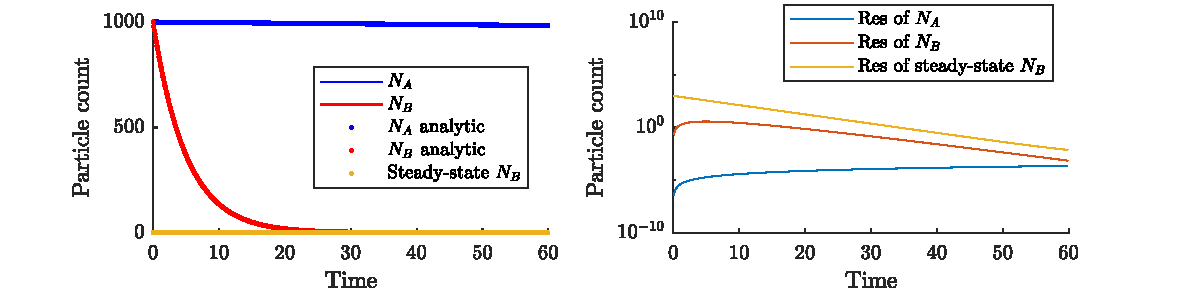
\includegraphics[width=0.7\linewidth]{largetau.pdf}
		\caption{\textbf{INSERT PURDY CAPTION PL0X}}
		\label{fig:largeTau}
	\end{figure}
	as seen, the steady-state solution for $ N_B $ (\eqref{eq:steadyNB}) does correctly predict the behaviour for $ N_B $, when this is approximately 0. This makes sense; the change in $ N_A $ is almost constant, corresponding to when $ N_B $ is approximately 0, which is the steady state for this particular problem.
	
	
	\section{Projectile motion}
	For this assignment, projectile motion is to be simulated, again using the Euler-method. This gives another example of how to use this simple method of simulation, for a problem which (without wind resistance) has an analytical solution. After this, uncharted waters are encountered, when wind resistance is included. Here no analytical solution is given, and all reliance upon the previous methods, like residuals between the numerical and analytical solutions, are not applicable.
	
	Furthermore, for this problem, a second derivative is used, whereby a second Euler integration is needed, to complete the time step. The relevant differential equations are
	\begin{equation}\label{key}
		\diff[\ud]{\V{r}}{t} = \V{v}, \quad \diff[\ud]{\V{v}}{t} = -g\Vy.
	\end{equation}
	where the analytical solution is computed by integrating the second equation twice, and using the relevant initial conditions:
	\begin{equation}\label{key}
		\V{r}(t) = \begin{pmatrix}
		x(t) \\ y(t)
		\end{pmatrix} = \begin{pmatrix}
		x_0+v_{x,0} t \\ y_0+v_{y,0}t-gt^2/2
		\end{pmatrix}. 
	\end{equation}
	
	
	\subsection{Without wind resistance}
	The numerical and analytical solutions to projectile motion, given the initial conditions of $ x_0 = 0,y_0 = 2 \e{m},v_0 = 4 \e{m/s}$ and $ \theta = 70\degree$, where $ v_{x,0} = v_0 \cos \theta $ and $ v_{y,0} = v_0 \sin \theta $. For the numerical solution a value of $ \Delta t = 0.01 \e{s}$ is used. The results are shown below, along with the absolute residual, as a function of time:
	\begin{figure}[H]
		\centering
		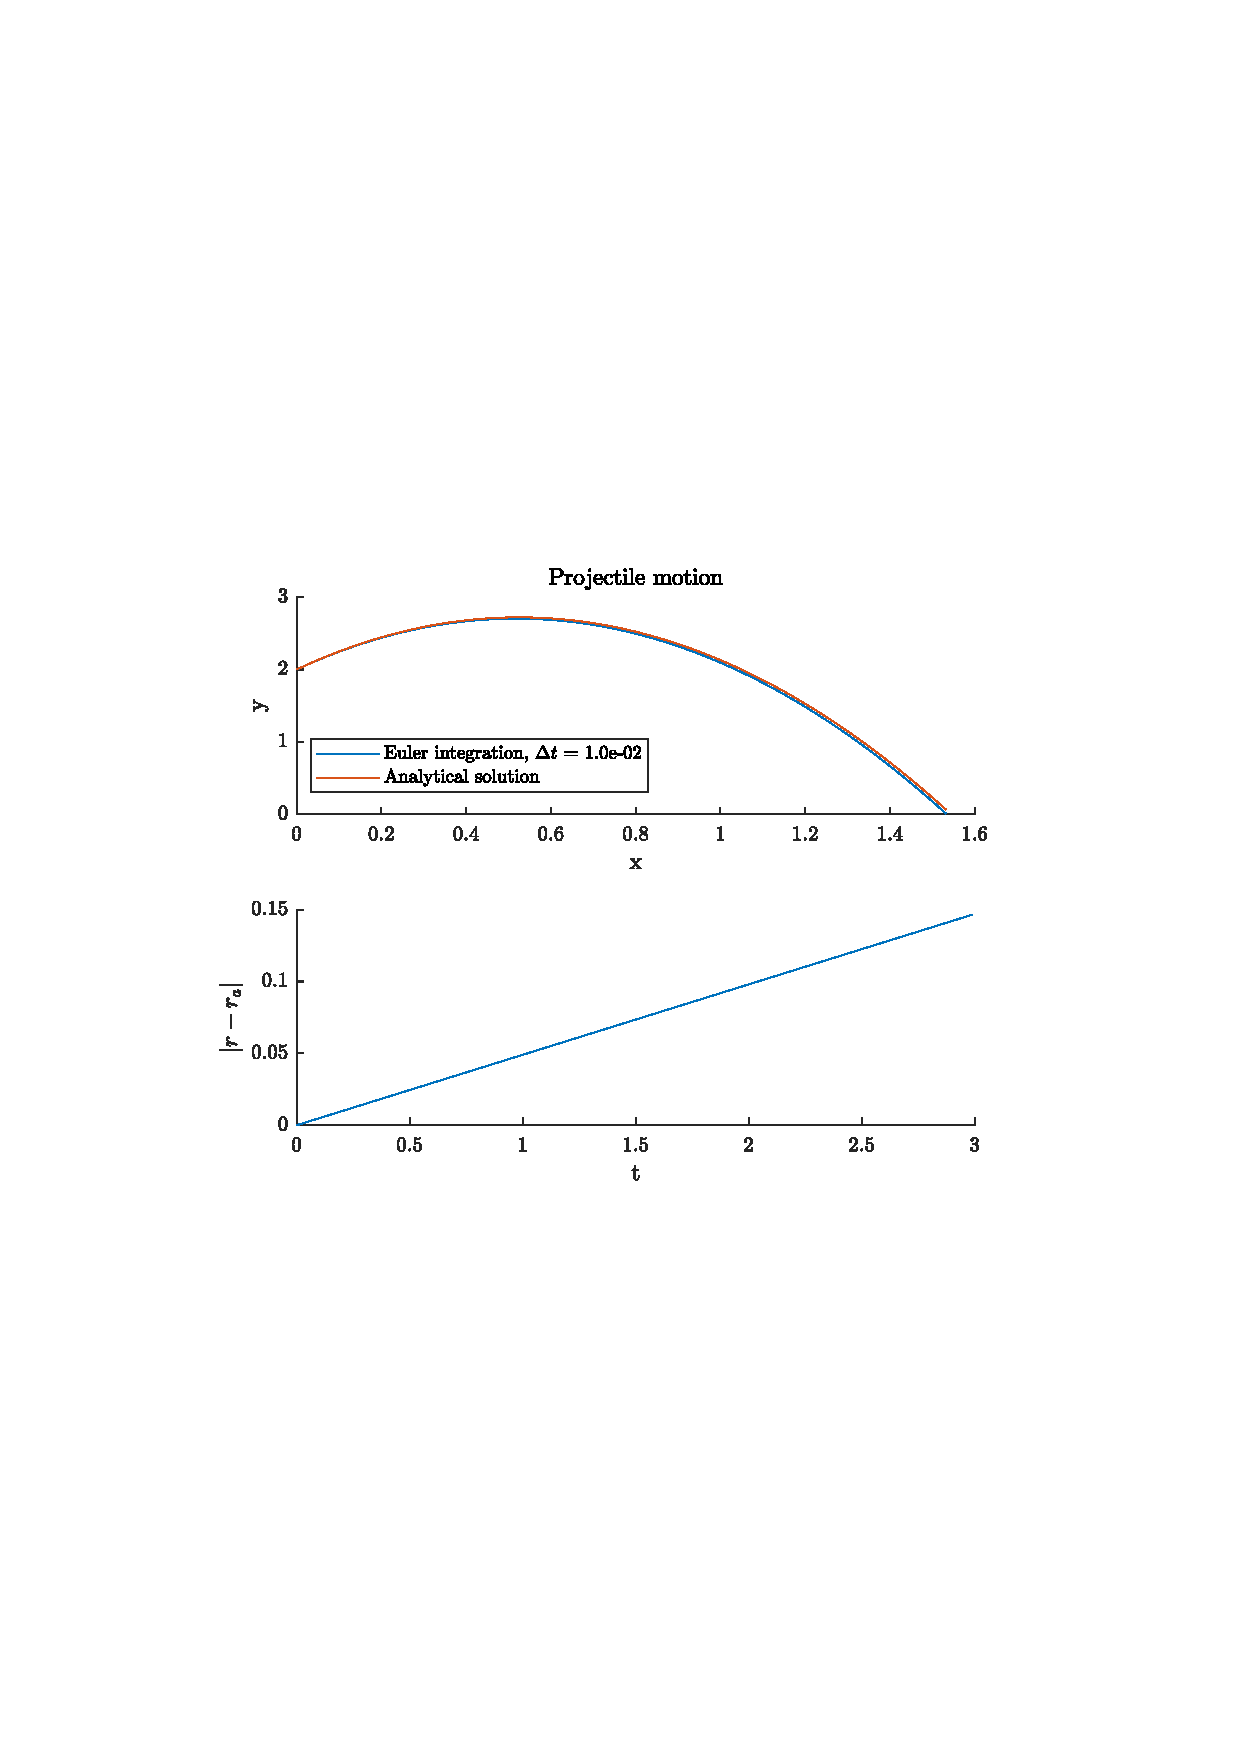
\includegraphics[width=0.7\linewidth]{projectile.pdf}
		\caption{\textbf{INSERT PURDY CAPTION PL0X}}
		\label{fig:projectile}
	\end{figure}
	the absolute residual is also the global truncation error, as defined in the slides for the week 1 lectures. As is expected, the error increases linearly in time, given the linear increase in velocity. This means that the Euler integration underestimates the velocity by a constant amount per time step, leading to a linear increase in global truncation error.
	
	
	
\end{document}

